\documentclass[11pt]{article}

\usepackage{amsmath}
\usepackage{amssymb}
\usepackage{fancyhdr}
\usepackage{isotope}
\usepackage{graphicx}
\graphicspath{{./images/}{./}}
\usepackage{array}
\usepackage{caption}
\usepackage{subcaption}

\oddsidemargin0cm
\topmargin-2cm     %I recommend adding these three lines to increase the 
\textwidth16.5cm   %amount of usable space on the page (and save trees)
\textheight23.5cm  

\newcommand{\question}[2] {\vspace{.25in} \hrule\vspace{0.5em}
\noindent{\bf #1: #2} \vspace{0.5em}
\hrule \vspace{.10in}}
\renewcommand{\part}[1] {\vspace{.10in} {\bf (#1)}}

\newcommand{\myname}{Matthew J. Urffer}
\newcommand{\myemail}{murffer@utk.edu}
\newcommand{\myhwnum}{3}

\pagestyle{fancyplain}
\lhead{\fancyplain{}{\textbf{HW\myhwnum}}}      % Note the different brackets!
\rhead{\fancyplain{}{\myname\\ \myemail}}
\chead{\fancyplain{}{CHEM-630}}

\begin{document}

\medskip                        % Skip a "medium" amount of space
                                % (latex determines what medium is)
                                % Also try: \bigskip, \littleskip

\thispagestyle{plain}
\begin{center}                  % Center the following lines
{\Large CHEM-630 Assignment \myhwnum} \\
\myname \\
\myemail \\
January 22, 2013 \\
\end{center}

\question{1.11}{Atoms}

%%%%%%%%%%%%%%%%%%%%%%%%%%%%%%%%%%%%%%%%%%%%%%%%%%%%%%%
\part{a}{Calculate the average atomic weight of the element when Ag has 51.35\% \isotope[107]{Ag} and \isotope[109]{Ag}}

\begin{align}
	<mass> &= 0.5135\times106.90508\text{mu} + (1-0.5135)\times108.90475\text{mu}\\
			 &= 107.85592\text{mu}
\end{align}
%%%%%%%%%%%%%%%%%%%%%%%%%%%%%%%%%%%%%%%%%%%%%%%%%%%%%%%
\part{b}{Identify an element which has 7 stable isotopes}

Ruthenium, dysprosium, ytterbium, and mercury all have 7 stable isotopes.

%%%%%%%%%%%%%%%%%%%%%%%%%%%%%%%%%%%%%%%%%%%%%%%%%%%%%%%
\part{c}{Identify a stable nuclide which shows wither a magic neutron number only or a magic proton number only. What sign of extra stability to you find in it?}

The magic nucleon numbers are 2,8,20,28,50,82 and 126.
A stable nuclide with a magic proton number of 8 is \isototope[18]{O}.  
In this isotope the 10 neutrons are paired up in even-even spin, and is therefore a more stable energy state than an even-odd paring.
Even-odd pairings would occur with the magic nucleon numbers since the magic nucleon numbers are all even.

%%%%%%%%%%%%%%%%%%%%%%%%%%%%%%%%%%%%%%%%%%%%%%%%%%%%%%%
\part{d}{Plat a graph of the average atomic weight of the elements up through Th minus the atomic number (avg atomic wt - Z) against the atomic number (Z). How is this line related to the stability band?}

Data was parsed from the 2007 atomic weights of the elements (IUPAC Technical Report) for the average atomic weight.
The Z of each element was then subtracted off the of the atomic weight, and plotted in Figure ~\ref{fig:StabilityBand}.
The resulting line is essentially the center of the stability band.
\begin{figure}[ht]
	\centering
	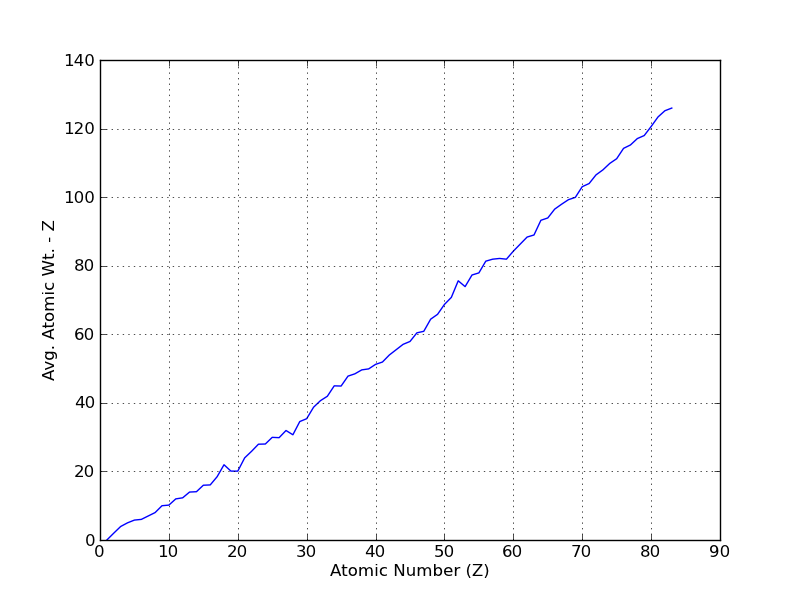
\includegraphics[width=\textwidth]{StabilityBand.png}
	\caption{Average Atomic Weight - Z}
	\label{fig:StabilityBand}
\end{figure}

%%%%%%%%%%%%%%%%%%%%%%%%%%%%%%%%%%%%%%%%%%%%%%%%%%%%%%%
\question{Advanced Topic}{Extended Periodic Table - Part 2, Binding Energy}

The binding energy per nucleon was investigated using the semi-empirical mass model along with published data.
For each A, Z the semi-empirical mass model was used to calculate the binding energy, with the results shown in the contour plot of Figure ~\ref{fig:BESemiEmperical}.
It is immediately evident why the heavy elements tend to have more isotopes, because their is a large plateau in the 8 MeV per nucleon range.
This plateau ends around a Z of 80, which is around where the elements have a high change of being radioactive.
In addition, the binding energy per nucleon starts to decline, indicating that according the the semi-empirical mass model that there is a finite number of elements\footnote{The coefficients of the semi-empirical mass model are from fitted data, so it probably should not be extrapolated very far}.
The semi-empirical binding energy per nucleon was compared to the published values from the NNDC\footnote{Data from http://www.nndc.bnl.gov/masses/mass.mas03}, and the log error between the two was calculated and shown in Figure ~\ref{fig:BEError}.
In general, there was very good agreement.  However, the real values did not show as much variability as the semi-empirical model. In addition, the semi-empirical model fails to capture the binding energy at very low A and Z, where quantum / shell models would be more accurate.
\end{document}

